\scanpage{107}

Or le deuxième mb est $\xi_0\underset{\substack{\Vert\\\xi_3}}{\bar\xi_0}\xi_1\underset{\substack{\Vert\\\xi_2}}{\bar\xi_1}$, or

\[
\begin{aligned}
\xi_0\bar\xi_0&\overset{!}{=}N_{A_1\otimes A_2/A}(\xi_0)\\
\xi_1\bar\xi_1&=N_{A_1\otimes A_2/A}(\underset{\substack{\Vert\\\sigma_1(\xi_0)}}{\xi_1})
=\overline{N_{A_1\otimes A_2/A}(\xi_0)}
\end{aligned}
\]

donc \deleted{\unsure{soit|si}} $N=N_{A_1\otimes A_2/A}(\xi_0)$, on trouve

\[
N\bar N=N_{A/\mathcal O}(N)\qquad\text{OK.}
\]

\figure{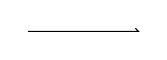
\begin{tikzpicture}\draw (0,0)--(1.4,0)--(1.36,.04);\end{tikzpicture}}

On va axiomatiser la situation de \deleted{\unsure{$A,A,\mathcal O$|$A,A_1,\mathcal O$}} $\mathrm{Tr}_{A_1\otimes A_2/A}$ et $N_{A_1\otimes A_2/A}$, en \unsure{considérant|explicitant|aboutit à|oubliant} la situation d'un anneau de base $k$, \inserted{et} d'une $k$-algèbre $A$ qui ``se comporte comme si c'\unsure{étais|était} une algèbre quadratique sur $k$'' (i.e. loc. libre de \unsure{rg|rang} $2$). Mais on ne suppose ni que $A$ soit loc. libre \deleted{\unsure{sur}} \inserted{ni $=$ plat} $/k$, ni que

\[
\alpha:k\longrightarrow A\qquad\lambda\longmapsto\lambda.1_A
\]

soit injective. Au lieu de cela, on suppose données \unsure{des|deux} applications

\[
\begin{aligned}
t_{A/k}=t &: A\longrightarrow k &\text{trace relative.}\\
n_{A/k}=n &: A\longrightarrow k &\text{norme relative,}
\end{aligned}
\]

satisfaisant les conditions suivantes

\textcircled{a} $t$ est linéaire, $n$ est quadratique, et $t$ se déduit de $n$ comme

\[
t(x)=\varphi_n(x,1)\qquad\text{$\varphi_n$ forme bil. ass. à $n$}
\]

donc on a \deleted{\unsure{équiv.}}

\[
\boxed{n(x+\unsure{\lambda_A|\lambda.1_A|\lambda1_A})=n(x)+\lambda^2\underset{\substack{\Vert\\1\ \text{cf. ci-dessous b)}}}{n(1)}+\lambda t(x)}
\]

% archive sheet number: 106

